\section{Datasets}
\label{sec:datasets}

Data for this report comes from different members of the consortium. The first dataset, is the one anticipated in the previous deliverable on data assimilation. It is generated by Giovanni Grassi (DC6) at CORIA and descibes a Hydrogen-Ammonia blend. This data contains different boundry conditions, making it suitable for pattern identification within the same phoenomena across different scenatios. Moreover the study of the behaviour of combustion of Hydrogen-Ammonia blends is extremely important in the scope of reducing NOx emission, one of the main objectives of the overall project.     
The second dataset is generated by Lorenzo Fracino (DC2) at RWTH Aachen and rapresents a Mehtane-Hydrogen mixing layer.  
\subsection{NH$_3$/H$_2$ non-premixed mixing layer}
\label{sec:DATA_CORIA}

This dataset consists of direct numerical simulations (DNS) of a two-dimensional non-premixed ammonia-hydrogen-air reacting mixing layer. It is generated by DCGIOVANNI at CORIA using the structured mesh reactive flow solver SiTCom-B \cite{sitcomb}. The configuration represents a splitter-plate stabilized flame in which a cold fuel stream and a hot air stream interact across a shear layer, representative of conditions encountered in practical burners. 

The lower stream consists of a NH$_3$/H$_2$ fuel blend (with 15\% H$_2$ by volume) at ambient temperature (300~K) with a mean velocity of 15~m~s$^{-1}$, while the upper stream consists of preheated air with a mean velocity of 39.6~m~s$^{-1}$. A cold wall maintained at 600~K is imposed at the top boundary, and a symmetry condition is applied at the bottom. Homogeneous velocity fluctuations of 10\% are prescribed at both inlets. The computational domain measures $12 \times 1$~cm and is discretized on a uniform grid of $2400 \times 200$ cells with a resolution of 50~$\mu$m. 

\FloatBarrier
\begin{figure}[htbp]
    \centering
    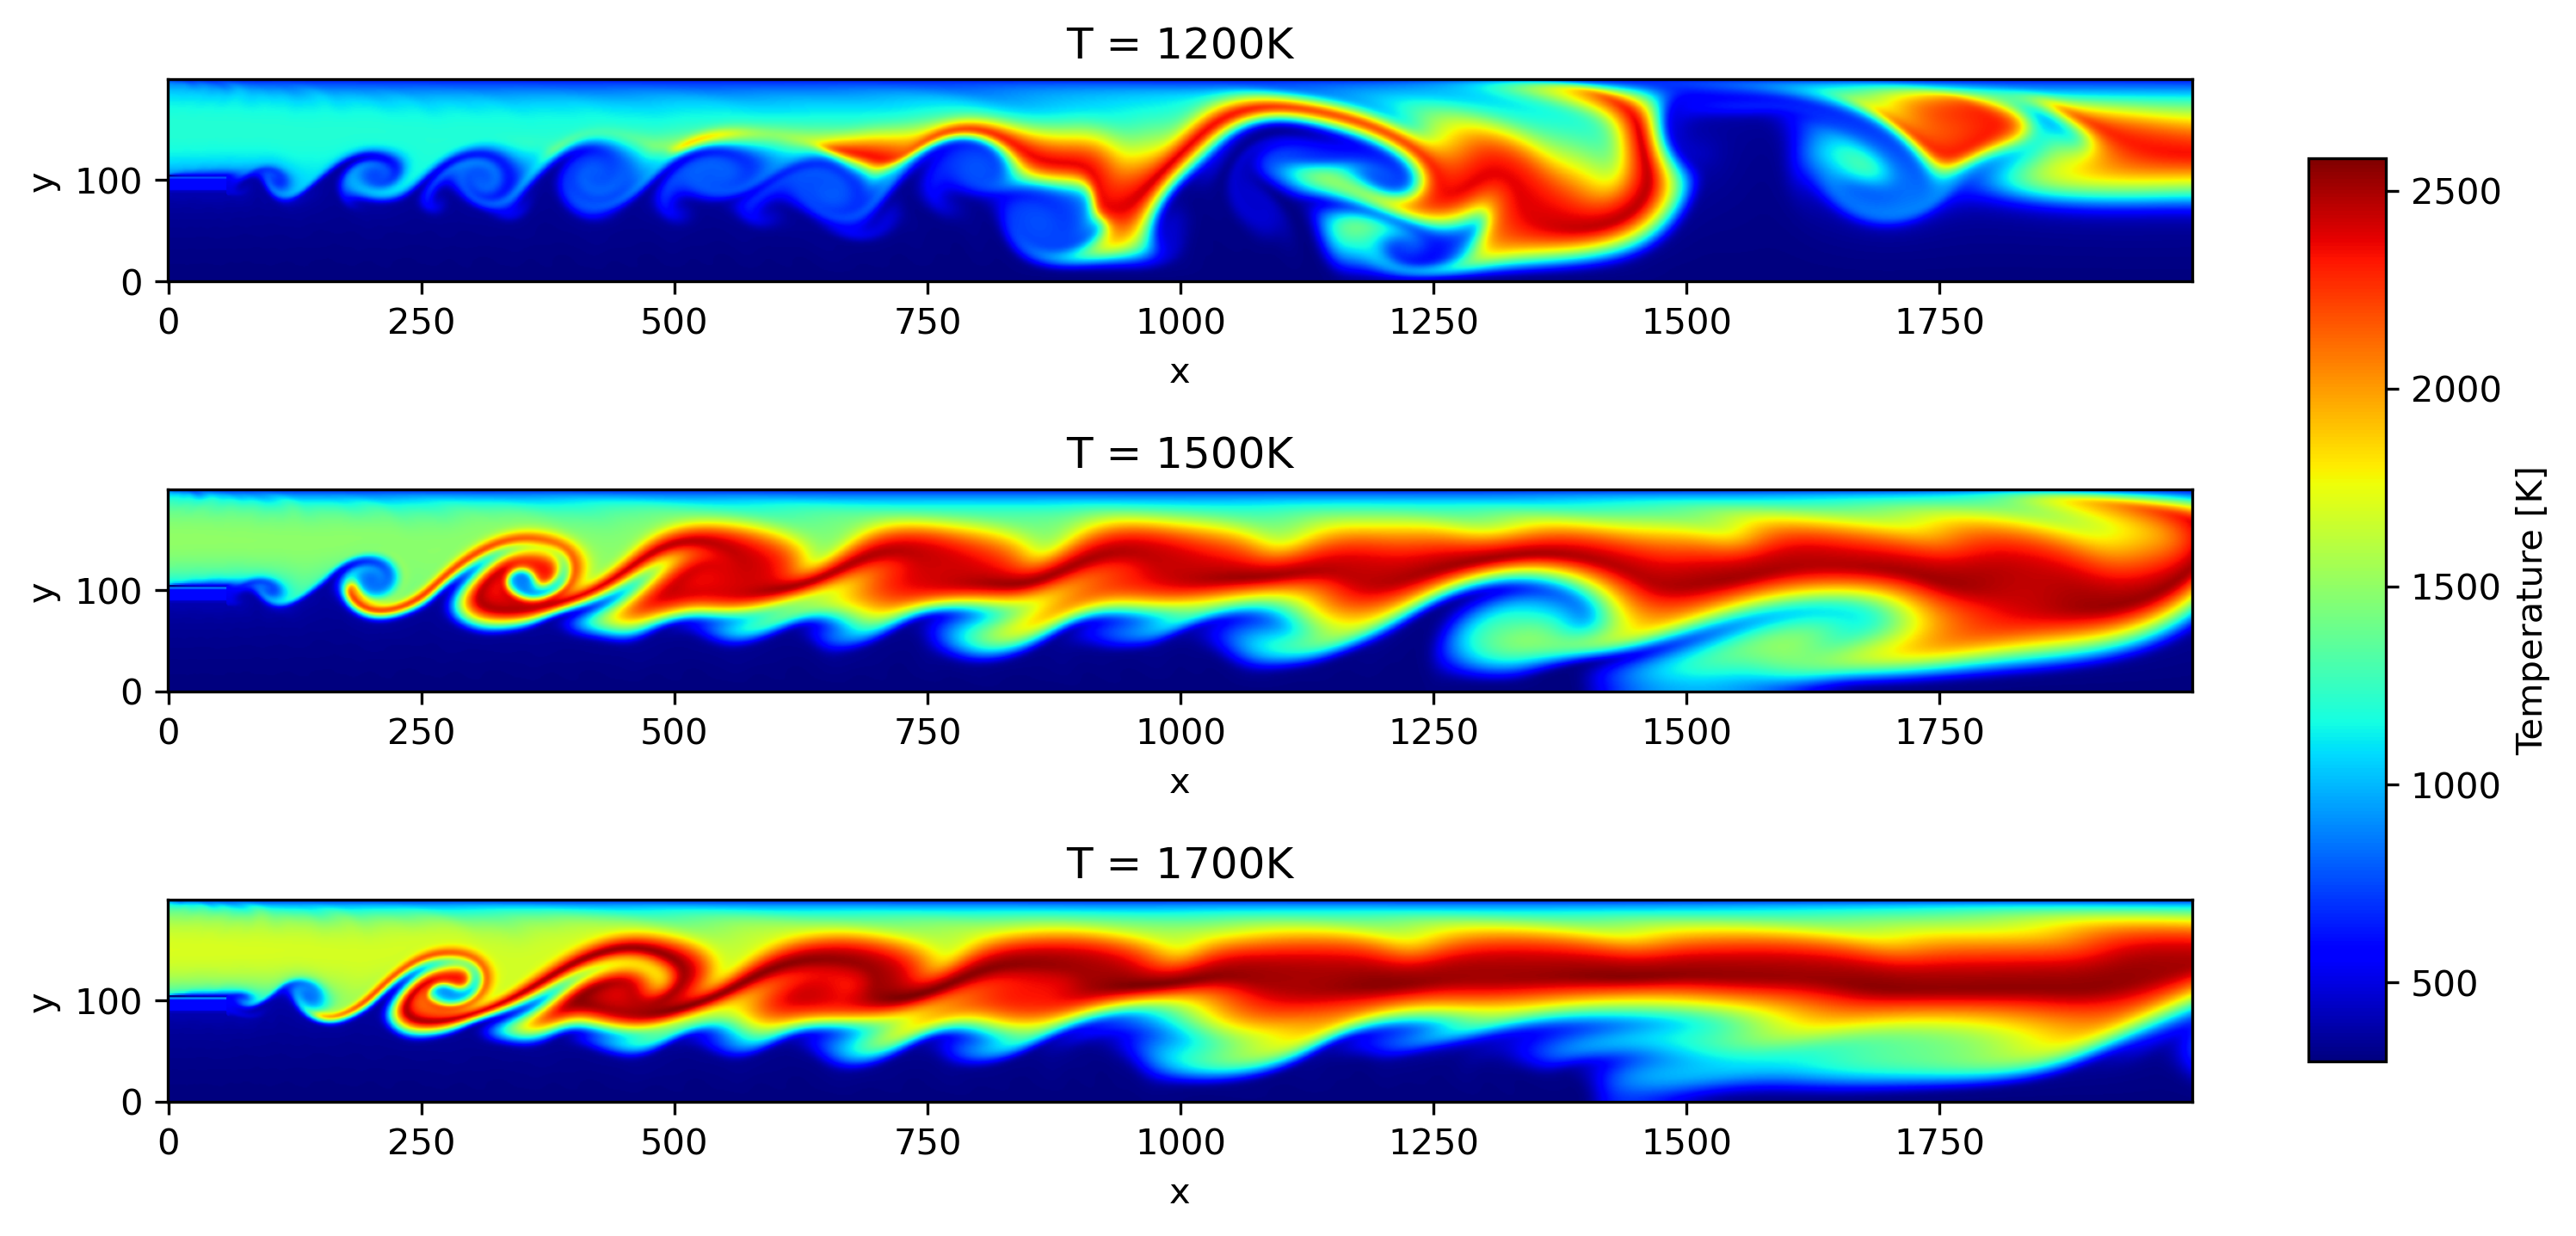
\includegraphics[width=0.85\textwidth]{../IMAGES/DATASETS/coria_3snap.png}
    \caption{Three representative snapshots of the temperature field from the NH$_3$/H$_2$ non-premixed reacting mixing layer DNS, illustrating the spatial evolution of the flame and mixing structures at different instants.}
    \label{fig:coria_data}
\end{figure}
\FloatBarrier

Three datasets are generated at different air preheat temperatures, namely 1200~K, 1500~K, and 1700~K, to probe the sensitivity of the flame dynamics and species evolution to the inlet thermal boundary condition. The domain geometry, grid resolution, and flow velocities are identical across all three cases. Each snapshot contains 19 reactive scalar fields corresponding to the species of the reduced mechanisms RmAH-1 and RmAH-2 \cite{grassi2025} — namely H$_2$, O$_2$, H$_2$O, H, O, OH, HO$_2$, NH$_3$, NH$_2$, NH, N, NO, NO$_2$, N$_2$O, HNO, NNH, N$_2$H$_2$, N$_2$, and Ar — together with temperature, yielding 20 variables in total. The species analysis presented in this work is conducted exclusively on the 1500~K dataset, which constitutes the reference operating condition for the assessment of the proposed methodologies.
\subsection{ULB hydrogen-fueled flameless furnace}
\label{sec:DATA_ULB}

This dataset comes from 2D CFD RANS of the ULB-modified stagnation-point reverse-flow combustor (SPRF) operating under flameless combustion conditions~\cite{giuntini2024continuously}. The domain is reduced to consider only the internal chamber of the burner. This choice was made to leave open the option of easily interpolating the data if necessary. The total number of available simulations is 175, but only 20 of them lie on a regular grid of operating conditions and are therefore suitable for an analysis with tensorial methods. This dataset is used to develop and validate the HOSVD+GPR reduced order model described in Section~\ref{sec:method_hosvd_gpr}.
The aforementioned grid is defined by three parameters: equivalence ratio $\phi$, hydrogen blending fraction in the fuel $H_2$, and operating pressure $p$:
\[
  \phi \in \{1.1,\,1.2,\,1.3,\,1.4,\,1.6\},
  \quad H_2 \in \{0.0,\,0.3\}\;\text{vol\%},
  \quad p \in \{1,\,2\}\;\text{atm}.
\]
These parameters are the ones that an operator can set before starting the combustion.

The data is arranged in a 5 dimensional tensor:
\[
  \mathcal{T} \;\in\; \mathbb{R}^{N_\phi \times N_{H_2} \times N_p \times N_{\mathrm{feat}} \times N_{\mathrm{cells}}},
\]
The analysis is performed solely on themorchemical variables, so temperature T and the 9 species $
\{N_2,\ NH_2,\ NO_2,\ H_2O,\ OH,\ O_2,\ H_2,\ NH_3,\ NO,\ T\}
$
indexed by $N_{\mathrm{feat}}$The 4 operating points with $\phi = 1.3$ are held out as the test set; the remaining 16 form the training set. 
Figure~\ref{fig:ulb_data} shows an example of one data point for a given operating condition ($\phi$ = 1.2, $H_2$ = 0.3 vol\%, $p$ = 2 atm ):
\FloatBarrier
\begin{figure}[htbp]
    \centering
    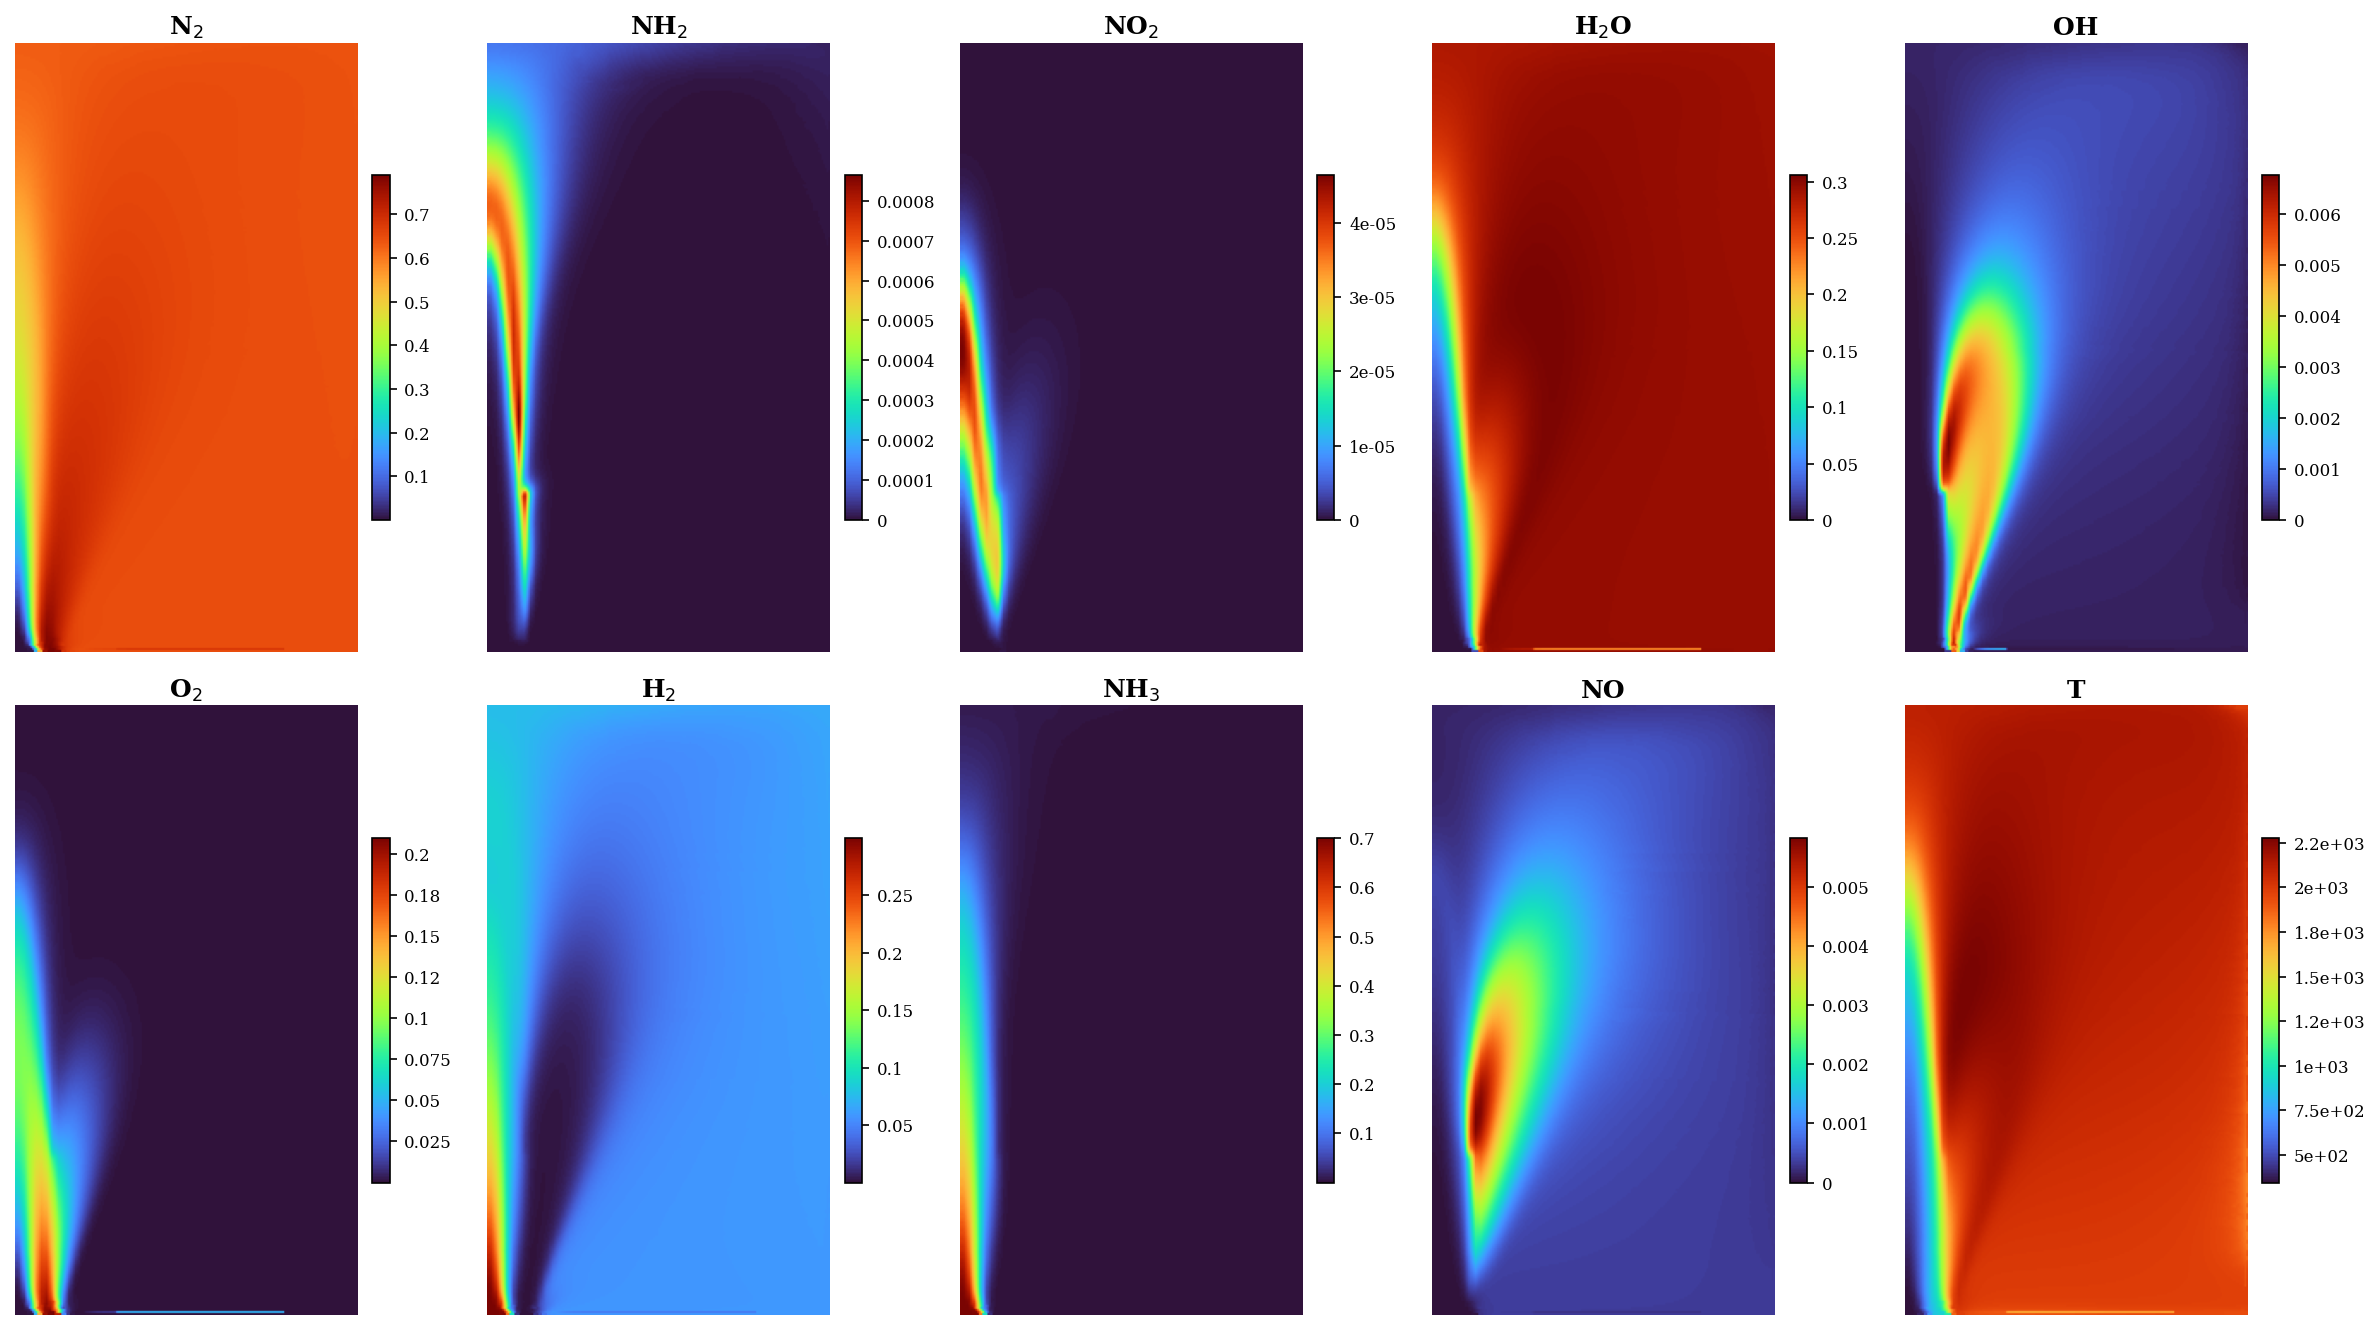
\includegraphics[width=0.85\textwidth]{../IMAGES/DATASETS/ulb_burner.png}
    \caption{Thermochemical variables of the ($\phi$ = 1.2, $H_2$ = 0.3 vol\%, $p$ = 2 atm) operating conditions point in the ULB-modified SPRF furnace.}
    \label{fig:ulb_data}
\end{figure}
\FloatBarrier
